% ================================
% Methodology
% ================================

\section*{Methodology}
\addcontentsline{toc}{section}{Methodology}

\subsection*{Research Design}
This study applies a qualitative, theory-building comparative case study design 
\parencite{George2005}. Germany and Chile are selected as ``most different systems'': 
both face similar biophysical pressures (droughts, wildfires, forest dieback) but 
are embedded in sharply contrasting political–institutional contexts. This design 
maximizes analytical leverage by showing how divergent legacies condition actor strategies.

\textbf{Germany} represents a corporatist welfare state with dense institutions 
and a tradition of consensus-oriented forestry.  
\textbf{Chile} exemplifies a fragmented neoliberal system with powerful 
private-sector actors and persistent socio-environmental conflicts.  
Comparing the two illuminates how institutional density versus fragmentation 
shapes bricolage strategies and uptake.

\subsection*{Operationalizing Observable Uptake}
Effectiveness of bricolage is defined through \textbf{observable uptake} in governance processes.  
Four indicators are coded:

\begin{enumerate}
    \item \textbf{Textual reuse in official drafts or laws.} Evidence of frames/instruments 
    appearing verbatim or paraphrased in legislation, decrees, or strategies. 
    \item \textbf{Resource allocation.} Clear link between proposals and funding (subsidies, 
    grants, pilot initiatives). 
    \item \textbf{Institutional incorporation.} Inclusion of bricolage elements in agency 
    mandates, procedures, or reporting frameworks. 
    \item \textbf{Actor representation.} Proponents gain seats or speaking roles in 
    decision-making venues (hearings, councils, advisory bodies). 
\end{enumerate}

\paragraph{Uptake Index weights.}
These four dimensions are reported \emph{disaggregated} and as a simple cumulative score (0–4).  
The cumulative score summarizes breadth, but does not imply equivalence (e.g., a law ≠ a 
hearing seat). Robustness checks test weighted alternatives (laws = 2; funding = 1.5) 
and an ordinal intensity scale (0–2). This prevents spurious equivalence and shows that 
findings are not artifacts of the index specification.

\paragraph{Negative uptake.}
Negative uptake is coded when a frame/instrument is explicitly rejected in official 
texts (e.g., ``inadmissible'', ``incompatible with X''). Rejections are treated as 1 
on a separate variable, ensuring that counter-mobilization is visible.

\paragraph{Timing.}
A lag variable records months between proposal and uptake, adding granularity 
to the analysis of how quickly bricolage diffuses.

\subsection*{Identifying Ideational Bricoleurs}
An actor (organization, coalition, or individual) is coded as a bricoleur when 
three \emph{observable} conditions are met:

\begin{enumerate}
    \item \textbf{Discursive recombination:} explicit combination of at least two 
    frames (e.g., ecological + justice; market + rights). 
    \item \textbf{Institutional patching:} linking or adapting instruments from 
    different domains (e.g., certification + indigenous co-management). 
    \item \textbf{Solution-framing:} presence of prescriptive markers such as 
    ``we propose'', ``should be implemented'', ``this measure will'', ensuring 
    only explicit problem–solution couplings are coded. 
\end{enumerate}

This avoids guessing ``intent'' and anchors classification in textual evidence.  
Modes of bricolage (layering, patching, transposition) are coded separately.  
Actors are stratified by type (state, NGO, business, science) to ensure comparability.

\subsection*{Auxiliary Frameworks}
Policy entrepreneurship, epistemic communities, and discourse coalitions are used 
\emph{only as boundary checks}. For instance, if bricolage clusters around individuals 
exploiting agenda windows, this is noted in memos (policy entrepreneurship), or if 
expert networks explain uptake, this is flagged (epistemic communities). These frameworks 
are not part of the core causal model, avoiding conceptual dilution.

\subsection*{Corpus Construction}
The corpus covers 2015–2025.  

\textbf{Primary corpus (30–40 docs/country):} high-salience laws, strategies, 
policy briefs from state, NGO, and industry actors.  
\textbf{Secondary corpus:} grey literature/media for context (not systematically coded).  

Inclusion: explicit forest adaptation/governance content; Exclusion: purely 
technical reports or duplicates.  

Search terms: DE (``Waldstrategie'', ``Anpassung Forst'', ``Borkenkäfer''),  
ES (``adaptación forestal'', ``Plan Nacional de Restauración''),  
EN (``forest adaptation'', ``ecosystem restoration'').  

Final sample: $\sim$65 documents (see Figure~\ref{fig:prisma}).  

\begin{figure}[h!]
\centering
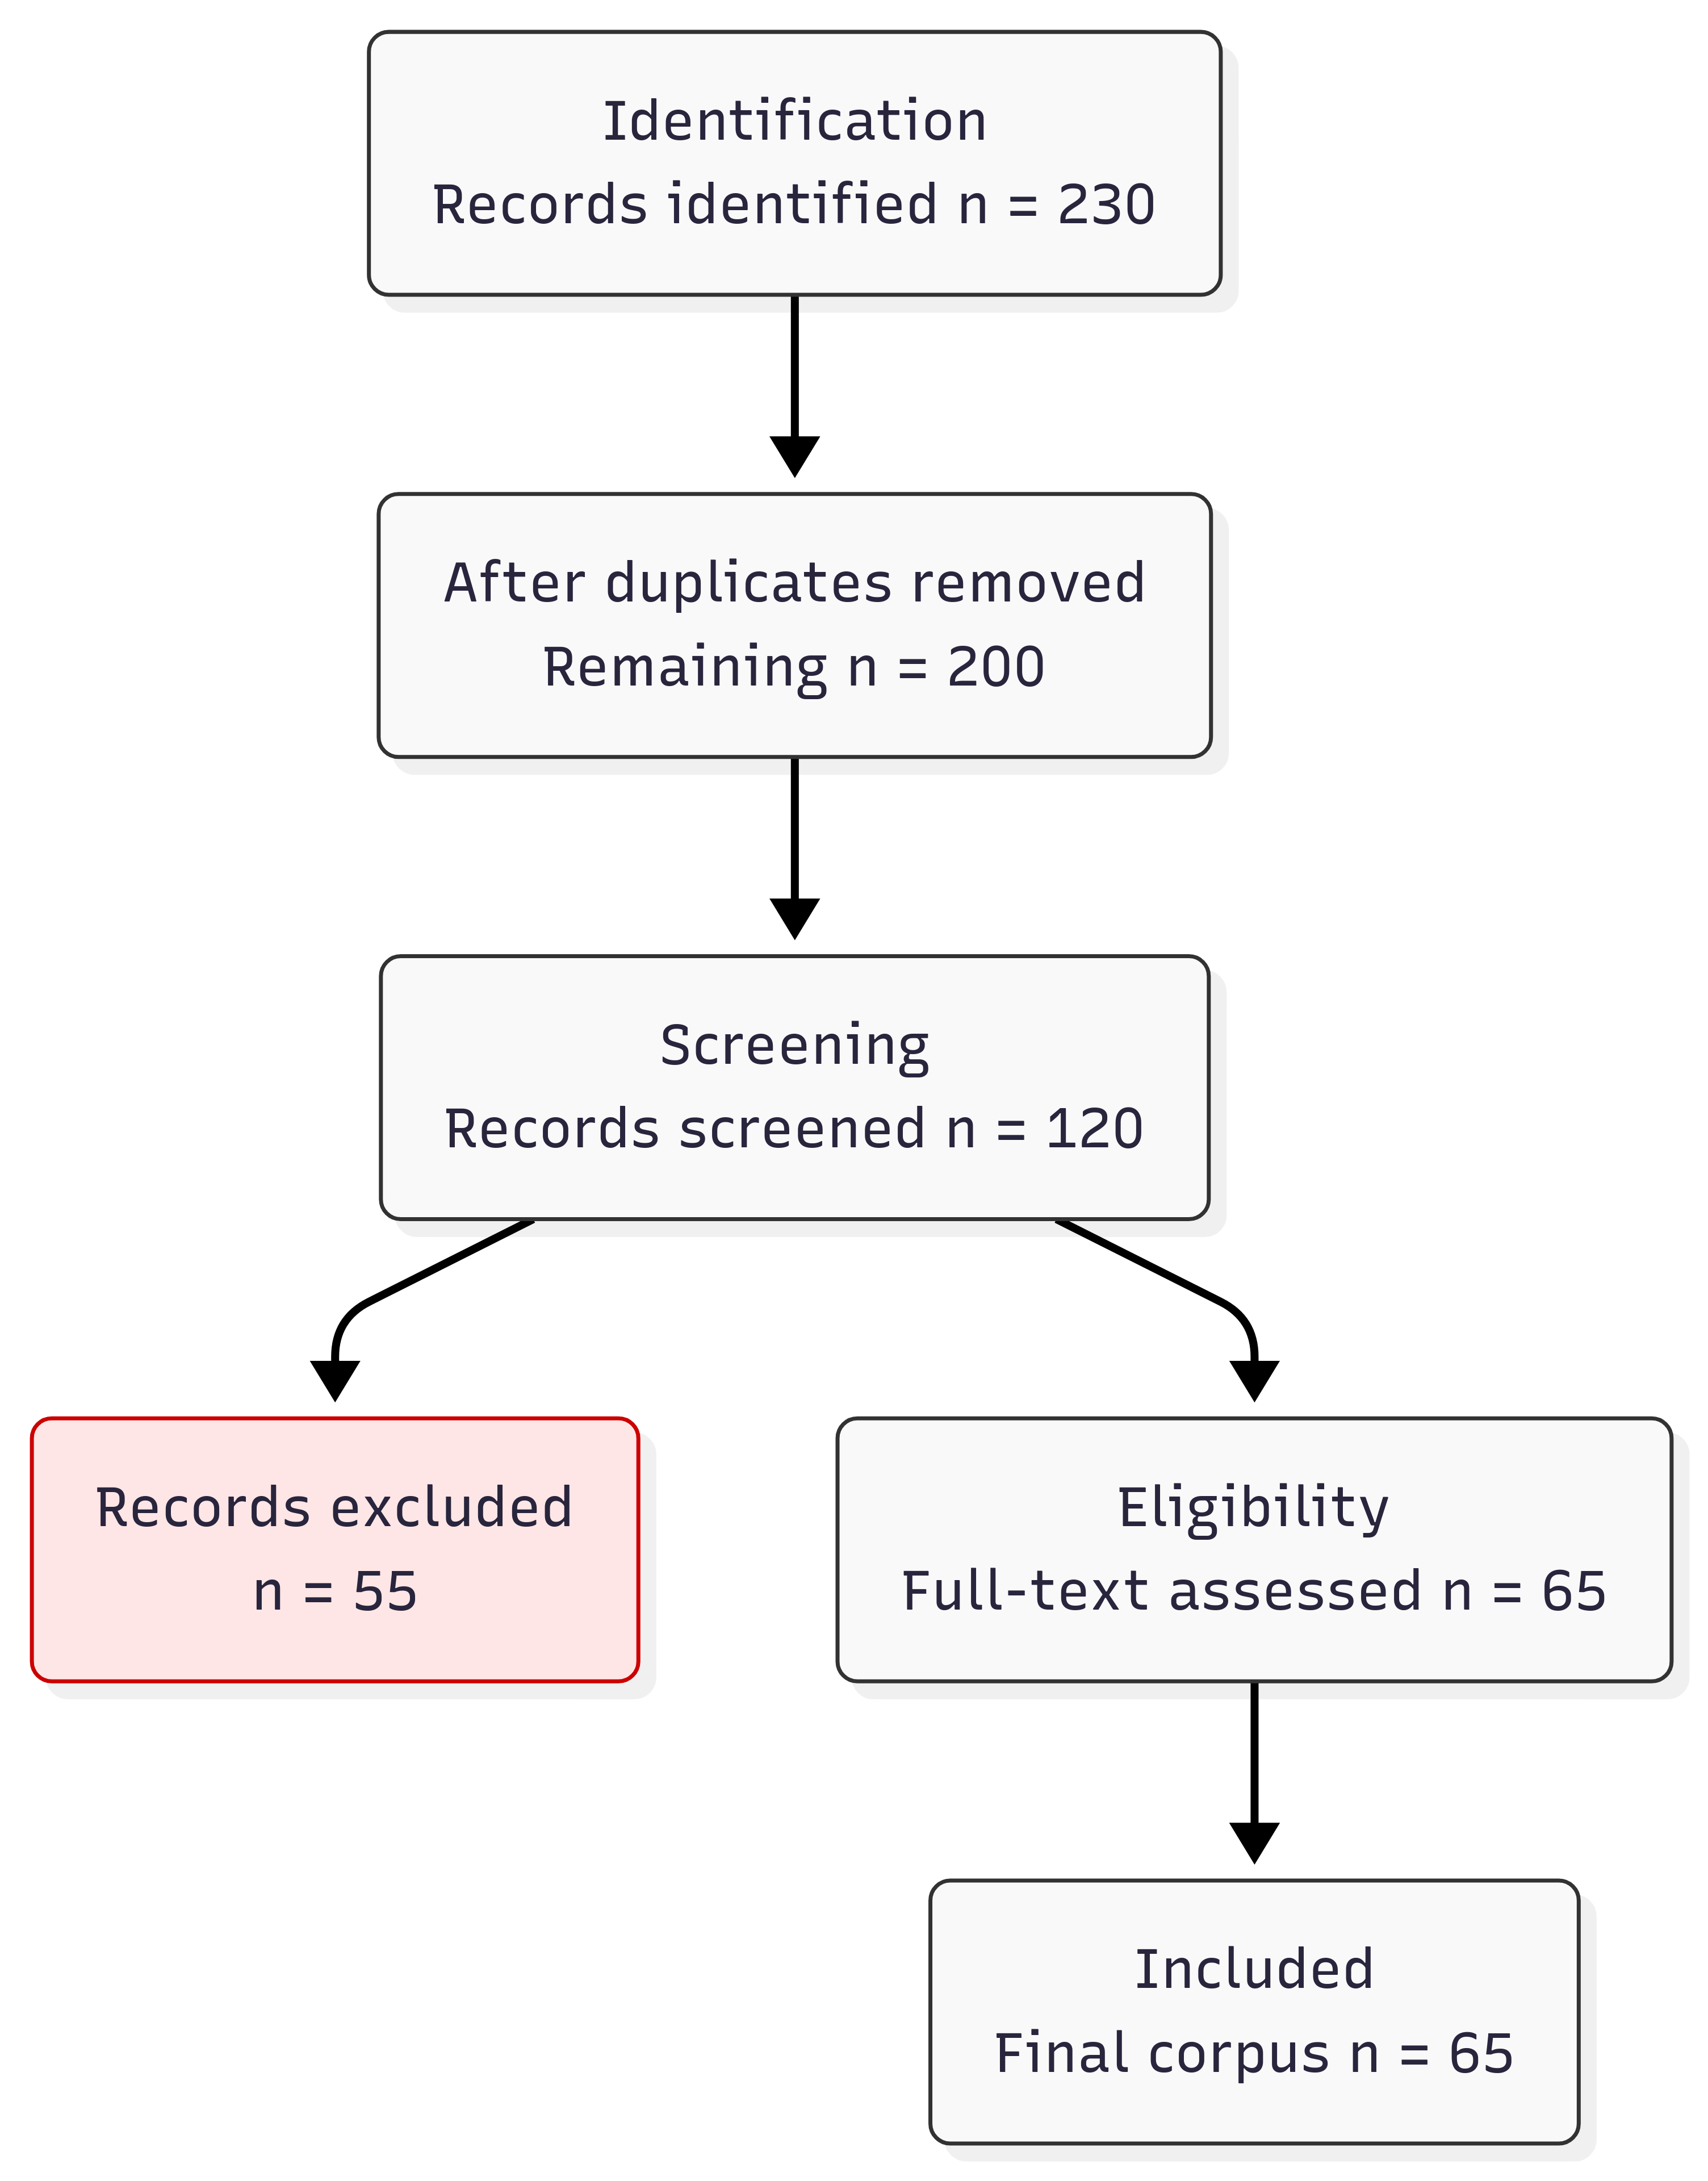
\includegraphics[width=0.8\textwidth]{src/fig/prop/06/prisma.png}
\caption{PRISMA flow diagram of document selection (final corpus $n=65$).}
\label{fig:prisma}
\end{figure}


\subsection*{Coding Protocol}
Documents are coded with a structured codebook:  
(1) Frames (diagnostic, prognostic, motivational),  
(2) Bricolage mode (layering, patching, transposition),  
(3) Uptake Index (0–4, + negative uptake, + timing).  

All coding decisions are memoed and version-controlled.

\subsection*{Reliability Strategy}
\begin{enumerate}
    \item Training round on 8–10 documents. 
    \item 25\% double-coded in both countries. 
    \item Cohen’s $\kappa$ reported (target ≥ 0.7). 
    \item Mid-project drift check + adjudication log. 
\end{enumerate}

\subsection*{Tools and Data Management}
Coding in \textbf{MAXQDA}, exported for transparency.  
Supplementary replicability checks in Python/R (text reuse detection, descriptive stats).  
All logs and metadata archived with version control.

\subsection*{Reflexivity and Safeguards}
\begin{itemize}
    \item Anonymized coding (first pass) to reduce reputational bias.  
    \item Adversarial memos: each bricolage instance paired with counter-interpretation.  
    \item Language awareness: coding in DE/ES; translation issues documented.  
\end{itemize}

The researcher’s dual background (Latin America + Europe) is both an asset and a 
risk; reflexive safeguards ensure this positionality informs interpretation 
without biasing coding.

\subsection*{Link to Hypotheses}
This design operationalizes H1–H3. Uptake distributions (H1/H2) are compared 
descriptively (medians, ranges, visualizations). Actor-type differences (H3) 
are shown via cross-tabulations. Results are stratified by venue type.  
The feedback loop in Figure~\ref{fig:causal} is treated as \emph{conceptual}: 
empirical analysis traces only the forward chain (frames $\rightarrow$ bricolage 
$\rightarrow$ uptake).